\documentclass[twoside,twocolumn]{article}
\usepackage{amsmath}
\usepackage{amsfonts}
\usepackage{amssymb}
\usepackage{graphicx}
\usepackage{blindtext} % Package to generate dummy text throughout this template 

\usepackage[hmarginratio=1:1,top=32mm,columnsep=20pt]{geometry} % Document margins
\usepackage[hang, small,labelfont=bf,up,textfont=it,up]{caption} % Custom captions under/above floats in tables or figures
\usepackage{booktabs} % Horizontal rules in tables
\usepackage{lettrine} % The lettrine is the first enlarged letter at the beginning of the text

\usepackage{enumitem} % Customized lists
\setlist[itemize]{noitemsep} % Make itemize lists more compact

\usepackage{abstract} % Allows abstract customization
\renewcommand{\abstractnamefont}{\normalfont\bfseries} % Set the "Abstract" text to bold
\renewcommand{\abstracttextfont}{\normalfont\small\itshape} % Set the abstract itself to small italic text

\usepackage{titlesec} % Allows customization of titles
\renewcommand\thesection{\Roman{section}} % Roman numerals for the sections
\renewcommand\thesubsection{\roman{subsection}} % roman numerals for subsections
\titleformat{\section}[block]{\large\scshape\centering}{\thesection.}{1em}{} % Change the look of the section titles
\titleformat{\subsection}[block]{\large}{\thesubsection.}{1em}{} % Change the look of the section titles

\usepackage{fancyhdr} % Headers and footers
\pagestyle{fancy} % All pages have headers and footers
\fancyhead{} % Blank out the default header
\fancyfoot{} % Blank out the default footer
\fancyhead[C]{Inteligencia de Negocios $\bullet$ Marzo 2021 $\bullet$ } % Custom header text
\fancyfoot[RO,LE]{\thepage} % Custom footer text

\usepackage{titling} % Customizing the title section

\usepackage{hyperref} % For hyperlinks in the PDF

%----------------------------------------------------------------------------------------
%	TITLE SECTION
%----------------------------------------------------------------------------------------

\setlength{\droptitle}{-4\baselineskip} % Move the title up

\pretitle{\begin{center}\Huge\bfseries} % Article title formatting
\posttitle{\end{center}} % Article title closing formatting
\title{Comparativa Analitica de Negocios vs Inteligencia de Negocios} % Article title
\author{Mamani Perez, LaTorre, Carpio Tejada ,Atahuachi Rivera, Velasquez Garcia}
\date{\today} % Leave empty to omit a date

\renewcommand{\maketitlehookd}
{%
\begin{abstract}
\noindent  La diferencia entre Inteligencia de Negocios y Analítica de negocios, es que la inteligencia de negocios crea reportes basados en el pasado y posibilita la toma de decisiones reactivas, mientras que la Analítica  de negocios se analiza el pasado para predecir el futuro y tomar decisiones proactivas. 

\end{abstract}
}
%----------------------------------------------------------------------------------------

\begin{document}

% Print the title
\maketitle

%----------------------------------------------------------------------------------------
%	ARTICLE CONTENTS
%----------------------------------------------------------------------------------------

\section{Introduccion}

\lettrine[nindent=0em,lines=2]{E}l análisis de datos permite saber cómo se comportan los clientes, qué quieren, en qué momento y cómo lo buscan. Con esta información, una compañía puede tomar decisiones inteligentes para mantener su rentabilidad y garantizar su competitividad. Si bien hay varias opciones disponibles para este propósito, las herramientas de Inteligencia de Negocios (BI) y de Analítica de Negocios (BA) son las soluciones de administración de datos más implementadas. Acompáñenos a despejar dudas y entérese cuál le conviene más a su compañía, cuál es el enfoque de cada una y qué tipo de soluciones aportan. 

%------------------------------------------------


%------------------------------------------------

\section{Desarrollo}

\subsection{ANALITICA DE NEGOCIOS}
Es el conjunto de métodos y técnicas utilizadas para trabajar como enlace entre los stackeholders, con el fin de comprender la estructura, políticas y operaciones de una organización y recomendar soluciones que permitan a la organización alcanzar sus objetivos.
 
\subsection{4  Aspectos de analisis de negocios}

\begin{figure}[h!]
	\centering
	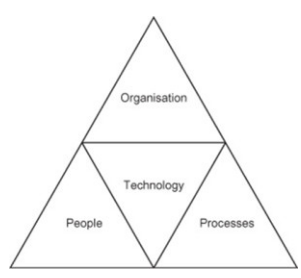
\includegraphics[scale=0.45]{Image/1.PNG}
	\caption{4 Aspectos de BA}
	\label{fig:Csha3}
\end{figure}

\begin{itemize}
\item[1]Los procesos:  
\newline
\item ¿están bien definidos y comunicados? ¿Hay buen soporte de TI, o existen varias soluciones? ¿El proceso requiere documentos que se pasean alrededor de la organización innecesariamente?
\newline
\item[2]Las personas: 
\newline
\newline
¿tienen las habilidades requeridas para el trabajo? ¿Qué tan motivados están? ¿Entienden los objetivos del negocio que tienen que soportar? 
\newline
\item[3]El contexto organizacional: 
\newline
\newline
 ¿hay un enfoque de gestión de apoyo? ¿Hay perfiles de cargo y responsabilidades bien definidas? ¿Hay trabajo interdisciplinario efectivo? 
\newline
\item[4]La tecnología: 
\newline
\newline
¿Los sistemas apoyan a la empresa como se requiere? ¿Ofrecen la información necesaria para dirigir la organización? 
\newline

\end{itemize}

\subsection{INTELIGENCIA DE NEGOCIOS}
\begin{itemize}
\item Combina análisis de negocios, minería de datos, visualización de datos, herramientas e infraestructura de datos, y las prácticas recomendadas para ayudar a las organizaciones a tomar decisiones más basadas en los datos. En la práctica, sabes que tienes una inteligencia de negocios moderna cuando tienes una visión integral de los datos de tu organización y los utilizas para impulsar el cambio, eliminar las ineficiencias y adaptarte rápidamente a los cambios del mercado o del suministro.
\newline
 
\end{itemize}
%--\includegraphics[width=6.5cm, height=4cm]{imagenes/Patrones creacionales/diagrama clases}
\subsection{Procesos y Actividades}
\begin{itemize}
	\item Minería de datos:
	\newline
	 Uso de bases de datos, estadísticas y aprendizaje automático para descubrir tendencias en grandes conjuntos de datos.
	\newline

		\item Generación de informes:
	\newline
	Comparar los datos de rendimiento actuales con los datos históricos para realizar un seguimiento del rendimiento en función de los objetivos, normalmente utilizando dashboards personalizados.
	\newline

		\item Análisis descriptivo:
	\newline
	Uso de análisis de datos preliminares para averiguar qué sucedió.
	\newline

		\item Generación de consultas:
	\newline
	Para extraer las respuestas de los conjuntos de datos, la BI hace preguntas específicas sobre los datos.
	\newline

		\item Análisis estadístico:
	\newline
	Tomar los resultados de análisis descriptivos y explorar aún más los datos utilizando estadísticas para determinar cómo sucedió esta tendencia y por qué.
	\newline

		\item Visualización de datos:
	\newline
	Convertir el análisis de datos en representaciones visuales como cuadros, gráficos e histogramas para consumir datos con mayor facilidad.
	\newline

		\item Análisis visual:
	\newline
	Explorar datos a través de la narración visual para comunicar ideas sobre la marcha y mantenerte dentro del flujo de análisis.
\newline

\item ¿Por qué es importante la inteligencia de negocios?
\newline

La inteligencia de negocios muestra datos actuales e históricos dentro de su contexto empresarial para que las empresas tomen mejores decisiones. Los analistas pueden aprovechar BI para proporcionar puntos de referencia de rendimiento y de la competencia para que la organización funcione de manera más fluida y eficiente. 
\newline

	\item [1] Algunas formas en que la inteligencia de negocios puede ayudar a las empresas a tomar decisiones más inteligentes basadas en los datos:
	\newline
	
		\item Identificar maneras de aumentar las ganancias
		\item Analizar el comportamiento del cliente
		\item Comparar datos con los competidores
		\item Rastrear el rendimiento
		\item Optimizar operaciones
		\item Predecir el éxito
		\item Identificar las tendencias del mercado
		\item Descubrir inconvenientes o problemas
		
		

\end{itemize}


\begin{itemize}

\item 


\section{COMPARATIVA BI Y BA}
La diferencia entre Inteligencia de Negocios y Analítica es que la primera crea reportes basados en el pasado y posibilita la toma de decisiones reactivas, con Analítica se analiza el pasado para predecir el futuro y tomar decisiones proactivas.
\newline
\newline
Inteligencia de Negocios es análisis de los datos obtenidos y Analítica de Negocios es predicción a partir de los datos obtenidos.
\newline
El objetivo de las dos metodologías es tomar decisiones de negocios basada en datos, se podría decir que el BI se preocupa por el qué y el cómo, no por el por qué. En cambio, el BA sí se pregunta por qué pasan las cosas para poder predecir futuros comportamientos o tendencias.
\newline
\newline
El BI examina los datos que se reportan en un formato que puede interpretarse de manera clara y rápida. Los paneles de control en tiempo real, por ejemplo, son un mecanismo de visualización muy útil, pues gracias a ellos los administradores pueden generar reportes integrales y precisos que contienen datos relevantes y procesables para tomar acción dentro de la compañía.
\newline

El BA usa análisis predictivo para resolver problemas antes de que ocurran, basándose en aplicaciones que centralizan información procedente de fuentes diversas, y permiten crear paneles con informes que facilitan el análisis desde múltiples perspectivas para optimizar diversos procesos.
\newline
\newline

\begin{figure}[h!]
	\centering
	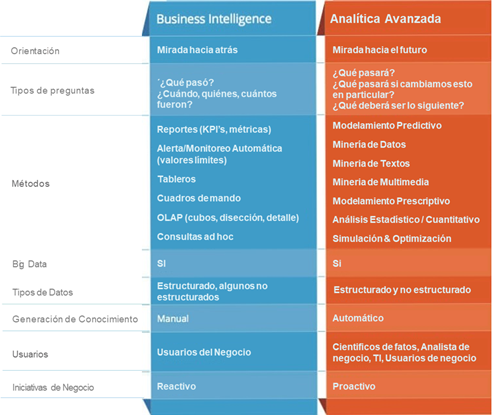
\includegraphics[scale=0.45]{Image/2.PNG}
	\caption{Comparativa BI vs BA}
	\label{fig:Csha3}
\end{figure}

\item {TIPOS DE SOFTWARE EN INTELIGENCIA DE NEGOCIOS }
\newline
\item	Microstrategy: 

Provee soluciones a clientes de cualquier industria o área funcional con el fin de ayudarlos en la obtención de un mayor conocimiento sobre la información manejada en su empresa .

\begin{figure}[h!]
	\centering
	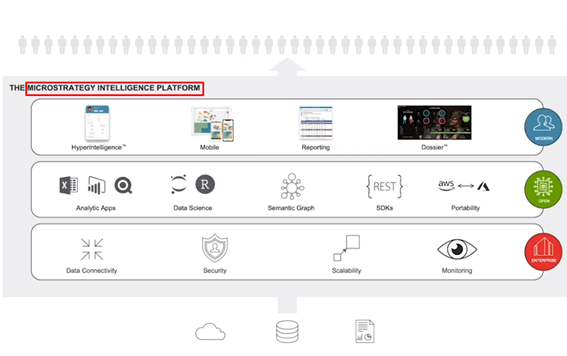
\includegraphics[scale=0.45]{Image/3.PNG}
	\caption{Microstrategy}
	\label{fig:Csha3}
\end{figure}


\item Bussiness objects: 

Suministra a los usuarios el poder acceder de forma sencilla a los datos ,analizar la información almacenada y creación de informes .
Su objetivo es convertir los datos de su organización en información útil y significativa, explotarla y, posteriormente, ser distribuida a aquellos que la necesitan, cuando la necesitan, para que puedan tomar decisiones oportunas.


\begin{figure}[h!]
	\centering
	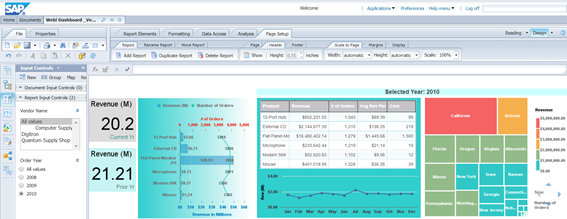
\includegraphics[scale=0.45]{Image/4.PNG}
	\caption{Bussines objects}
	\label{fig:Csha3}
\end{figure}


\item Cognos: 

Es un software que ofrece la funcionalidad de análisis y la toma de decisiones.
Para empresas que necesitan modelos predictivos, aumentar la capacidad de trabajo y la gestión de datos (analytics governance) acorde a sus necesidades, ya sea on-premises o en la nube. La plataforma que COGNOS utiliza para la construcción de soluciones de inteligencia de negocios (BI) esta basada en un framework de trabajo denominado UDW (Universal Data Warehose) que compila un conjunto de modelos y herramientas de trabajo resultantes del conocimiento de COGNOS ganado en el tiempo con la experiencia, el estudio y las certificaciones.


\begin{figure}[h!]
	\centering
	
\includegraphics[scale=0.45]{Image/5.PNG}
	\caption{Cognos}
	\label{fig:Csha3}
\end{figure}

\item 	oracle :

Permite acceder ,analizar y compartir la información para toma de decisiones bien precisas. 
La suite de BI Oracle sigue la nomenclatura de las diferentes ediciones de bases de datos que ya conocemos, por lo que ayuda mucho si ya estamos familiarizados con ella. Tenemos una Oracle BI Standard Edition 1 (BISE1), que es la más modesta y orientada a pymes. Después viene la Oracle BI Standard Edition (BISE), que en teoría correspondería a la versión intermedia. La versión más completa es la Oracle BI Enterprise Edition Plus (BIEE), orientada a la gran empresa.



\begin{figure}[h!]
	\centering
	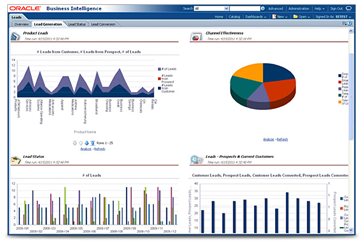
\includegraphics[scale=0.45]{Image/6.PNG}
	\caption{Oracle}
	\label{fig:Csha3}
\end{figure}

\item {HERRAMIENTAS PARA ANALISIS DE NEGOCIOS }
\newline
\item	Power BI:
Está pensada para que los equipos trabajen de forma colaborativa y presenta una amplia gama de plantillas y distintas opciones de visualización. Además, permite crear cuadros interactivos y gráficos, a partir de los datos de cada compañía. Entre sus principales ventajas también se encuentran la posibilidad de integrar a los usuarios a sus aplicaciones, que proporciona informes y cuadros de mando en tiempo real, que el equipo de IT tiene autonomía para administrar su sistema y que dispone de un excelente entorno gráfico de extracción, transformación y carga de información.

\begin{figure}[h!]
	\centering
	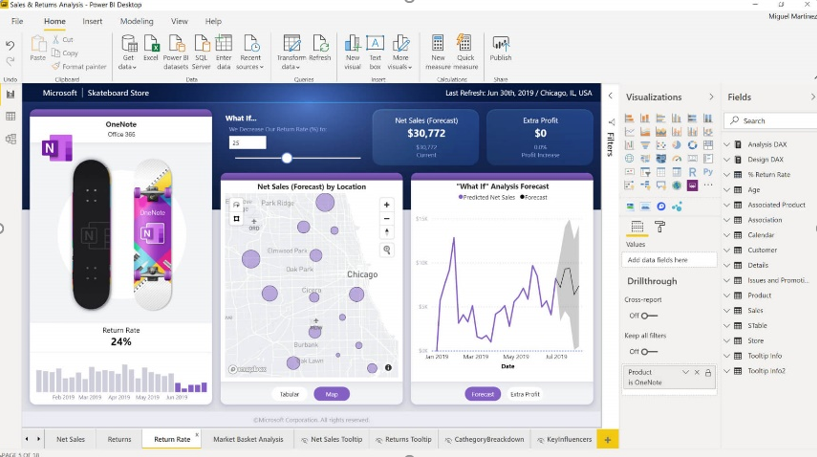
\includegraphics[scale=0.45]{Image/c7.PNG}
	\caption{Power BI}
	\label{fig:Csha3}
\end{figure}

\item	Tableau:
Uno de los programas líderes de análisis de datos y funciona, también, como una solución de análisis integral basada en la nube. El punto fuerte de esta herramienta es su tabla y el gráfico dinámicos de Excel. Su diseño, color e interfaz de usuario dan una sensación simple y fresca. Está diseñada para ayudar al usuario a tomar mejores decisiones sobre la forma más eficiente de extraer y comunicar el significado de los datos.

\begin{figure}[h!]
	\centering
	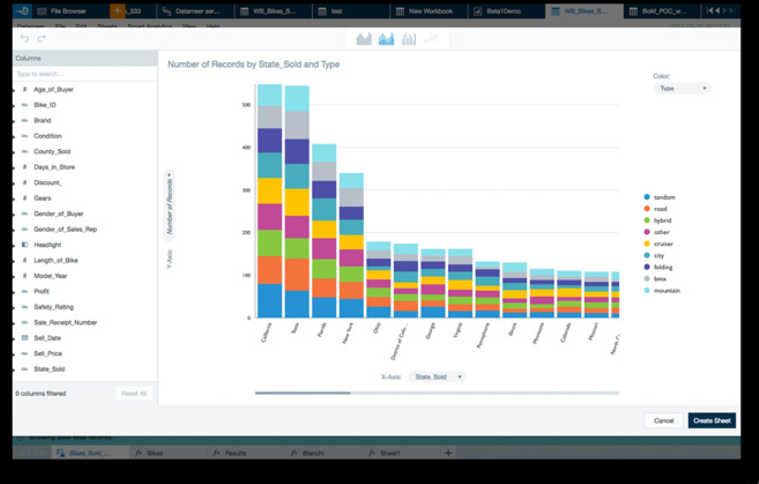
\includegraphics[scale=0.45]{Image/c8.PNG}
	\caption{Tableau}
	\label{fig:Csha3}
\end{figure}


\item	Geckoboard: 
Un programa que permite optimizar los datos de hojas de cálculo y bases de datos, a la vez que nos deja realizar presentaciones de una manera más clara y sencilla. Las métricas en tiempo real son fáciles de ver y entender, por lo que los equipos de trabajo podrán ver el impacto de sus ventas al instante. Dispone de más de 60 recursos y, en ella, es muy fácil crear dashboards. Además, permite filtrar los datos para mostrar exactamente lo que buscamos y su interfaz de usuario es muy intuitivo.
\newline
\item Qlik:
Se trata de una herramienta que utilizan más de 50.000 clientes en todo el mundo y que permite encontrar oportunidades únicas de negocio en el mercado online gracias a su software de Inteligencia Empresarial. Esta plataforma ofrece a sus usuarios descubrimientos de datos únicos a través de una búsqueda global de data, permite importar data a través de fuentes como Salesforce, Teradata y Hive, y nos da el control total de nuestros datos para elaborar informes y exportarlos en software amigables como los de Microsoft Office.

\begin{figure}[h!]
	\centering
	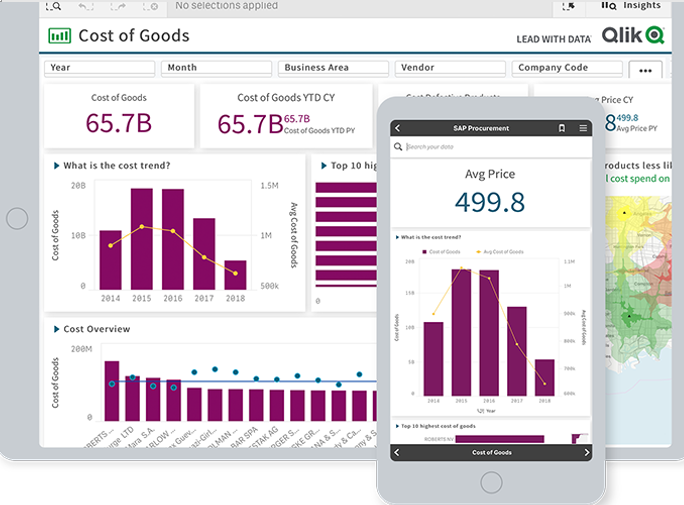
\includegraphics[scale=0.45]{Image/c9.PNG}
	\caption{Qlik}
	\label{fig:Csha3}
\end{figure}


\item Dundas BI:
Es una herramienta de Business Inteligence flexible que permite a los usuarios conectarse a múltiples fuentes de datos en tiempo real. Es el programa perfecto si lo que más nos interesa es la representación de datos para las diferentes áreas de nuestra empresa. Entre sus ventajas se encuentra su excelente organización y presentación en tablas, cuadros y gráficos de datos, la facilidad para crear informes propios solo con los KPI’s que nos interesen, y una buena experiencia de usuario en desktop, iPad y móviles.

\begin{figure}[h!]
	\centering
	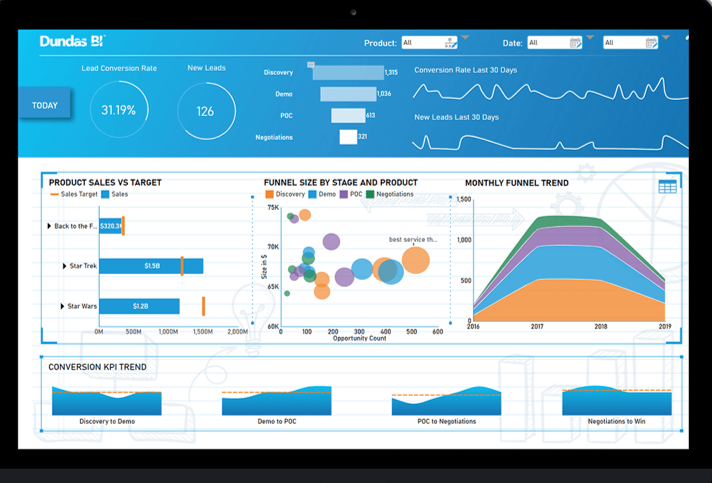
\includegraphics[scale=0.45]{Image/c10.PNG}
	\caption{Dundas BI}
	\label{fig:Csha3}
\end{figure}



\item Grow:
Esta herramienta permite importar y transformar fácilmente datos de múltiples fuentes para alimentar métricas y el panel de control. Cualquier usuario comercial puede crear métricas de forma intuitiva, filtrando, dividiendo y explorando diferentes tipos de gráficos a medida que navega por los datos. 

\begin{figure}[h!]
	\centering
	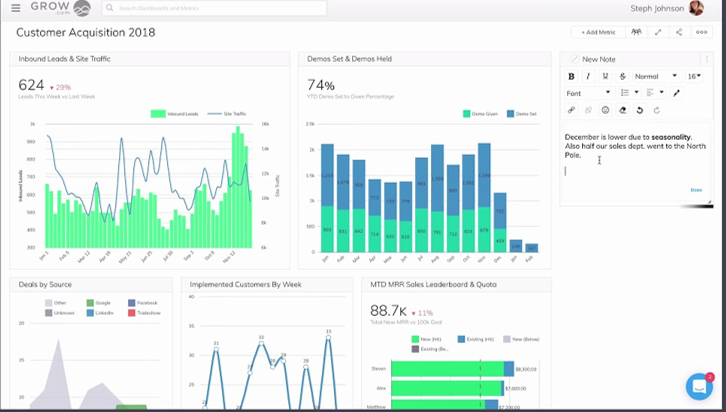
\includegraphics[scale=0.45]{Image/c11.PNG}
	\caption{Grow}
	\label{fig:Csha3}
\end{figure}

\section{Conclusiones}
En conclusion ambas son un complemento natural ya que requieren datos y prepararlos para hacer sus análisis y presentar resultados.
\newline
Los reportes pueden ser tanto de lo que ya ocurrió como de lo que se prevé que pasará.

\section{Recomendaciones}
Se recomienda comprender estos conceptos,ya que es vital para tomar las mejores decisiones comerciales, mantener una ventaja competitiva en todas las industrias y permitir que las empresas capturen valor operativo y estratégico.


\section{Bibliográfia}
\item Autor: Ramiro Ortega Juarez(2020).
\newline
\newline
Titulo: Introduccion a la Inteligencia de negocios.
\newline
\newline
\item Autor: Jose Lopez Arteaga(2019).
\newline
\newline
Titulo: Desarrollo de la Analitica de negocios e Inteligencia de Negocios.
\newline
\newline

\item Autor: Javiero Orrillo(2019).
\newline
\newline
Titulo: Analítica de negocios: Una estrategia basada en la información
\newline
\newline
Recuperado:https://www.esan.edu.pe/con-
exion/actualidad/2018/03/22/analitica-negocios-informacion/
\newline
\item Autor: Pedro Ruben FJ(2020).
\newline
\newline
Titulo: Diferencias entre Analisis de negocios y analitica de negocios.
\newline
\newline
Recuperado:https://business-intelligence.grupobit.net/blog/cual-es-la-diferencia-entre-business-intelligence-y-business-analytics


\item Autor: Juber F.(2020).
\newline
\newline
Titulo: Analisis de datos BI.
\newline
\newline
Recuperado:http://www.blog.dti-consultores.com/wp/2017/04/18/oracle-b-i-business-intelligence/

\item Autor: Jhonantan P.(2020).
\newline
\newline
Titulo: Oracle bussiness Intelligence.
\newline
\newline
Recuperado:http://www.blog.dti-consultores.com/wp/2017/04/18/oracle-b-i-business-intelligence

\item Autor: Romulo JP.(2020).
\newline
\newline
Titulo: Tableu bussiness Intelligence.
\newline
\newline
Recuperado:https://www.tableau.com/es-mx/learn/articles/business-intelligence


\item Autor: Enrique LM.(2019).
\newline
\newline
Titulo: Comparativa Business Intelligence vs Business Analytics.
\newline
\newline
Recuperado:https://www.esan.edu.pe/conexion/
actualidad/2018/03/22/analitica-negocios-informacion/


\item Autor: Andre Reynoso.
\newline
\newline
Titulo: Comparativa Business Intelligence vs Business Analytics.
\newline
\newline
Recuperado:https://github.com/Andre-Reinoso/Trabajo-Encargado-01-Comparativa-Business-Intelligence-vs-Business-Analytics


\item Autor: Jason Q (2019).
\newline
\newline
Titulo: Business Intelligence vs Business Analytics.
\newline
\newline
Recuperado:https://telemetrik.co/analitica-big-data-inteligencia-de-negocio-business-intelligence/


\end{itemize}
|\end{document}